\documentclass[11pt]{article}
\usepackage[margin=1in]{geometry}
\usepackage{amsmath,amssymb,amsthm,mathrsfs}
\usepackage{graphicx}
\usepackage[hidelinks]{hyperref}

\newtheorem{theorem}{Theorem}
\newtheorem{lemma}{Lemma}
\newtheorem{remark}{Remark}

\newcommand{\B}{\mathscr{B}}
\newcommand{\F}{\mathscr{F}}
\newcommand{\K}{\mathscr{K}}
\newcommand{\E}{\mathscr{E}}
\newcommand{\W}{\mathscr{W}}
\newcommand{\Linfty}{\ell_\infty}

\title{A positive answer to Dales Question (II) for \(c_0\oplus\ell_\infty\)}
\author{Smoke-test packet for \texttt{fa\_banach\_001}}
\date{2026-06-14}

\begin{document}
\maketitle

\section*{Status}

This packet claims a full solution of the specific subquestion in
Dales--Kania--Kochanek--Koszmider--Laustsen \cite{DKKKL}: for
\[
  E=c_0\oplus \ell_\infty,
\]
every finitely-generated maximal left ideal of \(\B(E)\) is fixed.  It does
not address the remaining \(C(K)\) cases in \cite{DKKKL}, such as
\(C[0,1]\) or \(C[0,\alpha]\) for \(\alpha\geq \omega^\omega\).

\section*{Source Question}

In \cite[Question (II)]{DKKKL}, Dales asks whether every
finitely-generated maximal left ideal of \(\B(E)\) is fixed.  The same paper
states on pages 23--24 that the answer was not known for
\(E=c_0\oplus\ell_\infty\).

\begin{center}
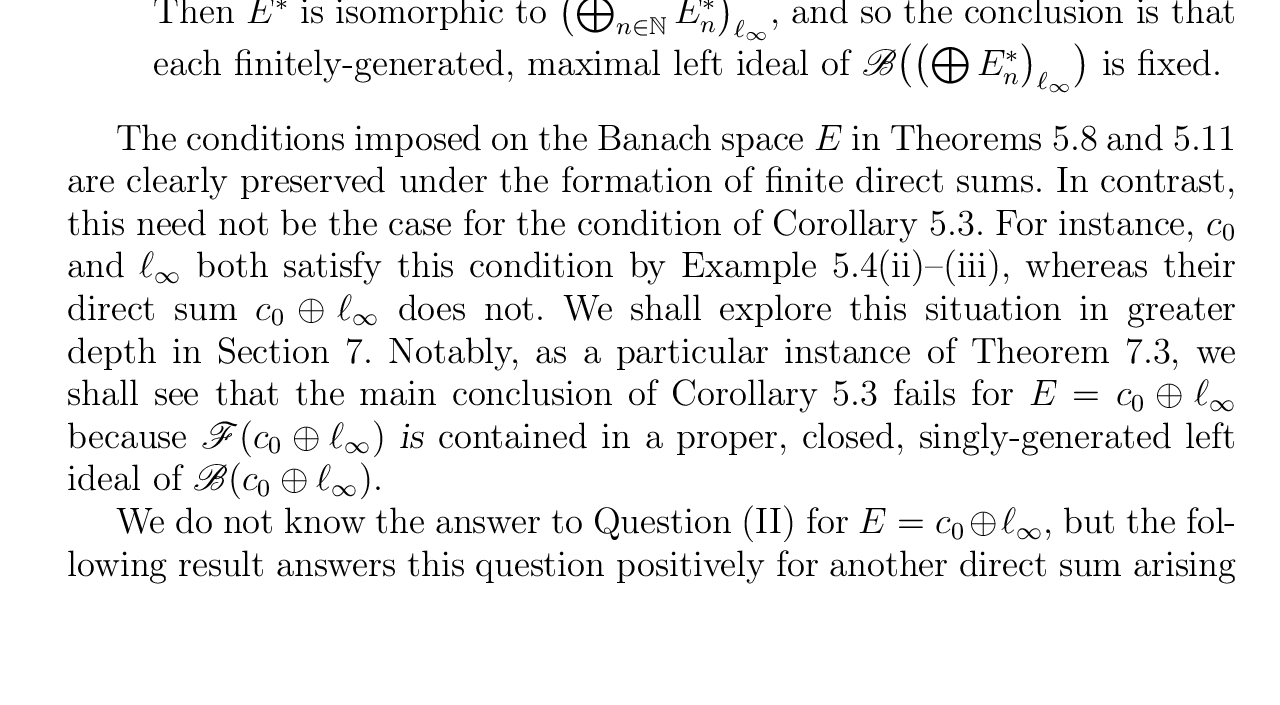
\includegraphics[width=\linewidth]{figures/open_problem_crop_page23.png}

\medskip
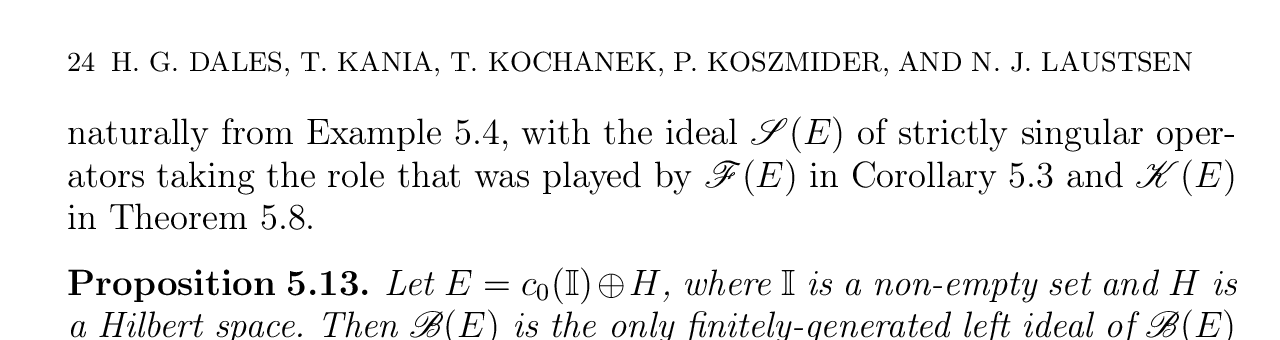
\includegraphics[width=\linewidth]{figures/open_problem_crop_page24.png}
\end{center}

\section*{Definitions and Source Inputs}

A maximal left ideal of \(\B(E)\) is fixed if it has the form
\[
  \mathscr{M}\mathscr{L}_x=\{T\in\B(E):Tx=0\}
\]
for some non-zero \(x\in E\).  We use the following results from
\cite{DKKKL}.

\begin{itemize}
\item The dichotomy theorem says that a non-fixed maximal left ideal contains
  \(\F(E)\).
\item The strong dichotomy, Corollary 4.1, says that a non-fixed maximal left
  ideal contains the ideal \(\E(E)\) of inessential operators.
\item Corollary 4.7 says that, for a finite generating family
  \(\Gamma\subset \B(E)\), containment \(\F(E)\subseteq \mathscr{L}_\Gamma\)
  is equivalent to the associated map
  \[
    \Psi_\Gamma:E\to E^{|\Gamma|},\qquad
    \Psi_\Gamma x=(Tx)_{T\in\Gamma},
  \]
  being bounded below.
\item Lemma 7.1 says that every operator \(\ell_\infty\to X\) is strictly
  singular whenever \(X\) contains no copy of \(\ell_\infty\).
\item Proposition 7.8 says that, for \(E=c_0\oplus\ell_\infty\), the ideal
  \[
    \K_1=
      \left\{
      \begin{pmatrix}
      A & B\\ C & D
      \end{pmatrix}\in \B(c_0\oplus\ell_\infty):
      A\in\K(c_0)
      \right\}
  \]
  is not contained in any finitely-generated maximal left ideal of \(\B(E)\).
\end{itemize}

\section*{Proof Intuition}

A non-fixed finitely-generated maximal left ideal \(L\) would contain
\(\F(E)\), so the finite generator map is bounded below.  Since
\(c_0\oplus\ell_\infty\) is isomorphic to each of its finite powers, this
places a bounded-below operator inside \(L\).  The strong dichotomy also
places all inessential operators inside \(L\).  For \(c_0\oplus\ell_\infty\),
the off-diagonal blocks are inessential, and the \(\ell_\infty\)-to-\(c_0\)
block of a bounded-below operator is strictly singular.  Therefore the lower
right block is upper semi-Fredholm, and injectivity of \(\ell_\infty\) lets
one manufacture the lower-right identity projection inside \(L\).  Together
with the inessential blocks this forces \(\K_1\subseteq L\), contradicting
Proposition 7.8 of the source paper.

\begin{lemma}\label{lem:k1-forced}
Let \(E=c_0\oplus \ell_\infty\).  If \(L\) is a non-fixed maximal left ideal
of \(\B(E)\) and \(L\) contains a bounded-below operator, then
\(\K_1\subseteq L\).
\end{lemma}

\begin{proof}
Write operators on \(E\) in block form relative to
\(E=c_0\oplus\ell_\infty\).  Since \(L\) is non-fixed, the strong dichotomy
\cite[Corollary 4.1]{DKKKL} gives \(\E(E)\subseteq L\).

We first record the block consequences.  Compact operators on \(c_0\) are
inessential.  Every operator \(\ell_\infty\to c_0\) is strictly singular by
\cite[Lemma 7.1]{DKKKL}, because \(c_0\) contains no copy of
\(\ell_\infty\); hence such operators are inessential.  By the standard
symmetry property for inessential operators, used in
\cite[proof of Theorem 7.7]{DKKKL} via Gonzalez \cite{Gonzalez}, every
operator \(c_0\to\ell_\infty\) is also inessential.  Finally, weakly compact
operators on \(\ell_\infty\) are inessential.  Thus \(L\) contains every block
matrix
\[
  \begin{pmatrix}
  A & B\\ C & D
  \end{pmatrix}
  \quad\text{with}\quad
  A\in\K(c_0),\ B\in\B(\ell_\infty,c_0),\
  C\in\B(c_0,\ell_\infty),\ D\in\W(\ell_\infty).
\]

Let
\[
  R=\begin{pmatrix} R_{11}&R_{12}\\ R_{21}&R_{22}\end{pmatrix}\in L
\]
be bounded below.  Restricting \(R\) to the \(\ell_\infty\)-summand shows
that the column map
\[
  y\mapsto (R_{12}y,R_{22}y),\qquad \ell_\infty\to c_0\oplus\ell_\infty,
\]
is bounded below, hence upper semi-Fredholm.  The operator \(R_{12}\) is
strictly singular, so stability of upper semi-Fredholm operators under
strictly singular perturbations gives that \(R_{22}\) is upper semi-Fredholm.

Choose a finite-rank projection \(Q\in\B(\ell_\infty)\) onto
\(\ker R_{22}\).  The restriction of \(R_{22}\) to \(\ker Q\) is an
isomorphism onto its closed range.  Since \(\ell_\infty\) is injective, the
inverse on \(R_{22}(\ker Q)\) extends to an operator
\(S\in\B(\ell_\infty)\), and so
\[
  SR_{22}=I_{\ell_\infty}-Q.
\]
As \(R\in L\), we have
\[
  \begin{pmatrix}0&0\\0&S\end{pmatrix}R
  =
  \begin{pmatrix}0&0\\ SR_{21}& I_{\ell_\infty}-Q\end{pmatrix}
  \in L.
\]
The off-diagonal block \(SR_{21}:c_0\to\ell_\infty\) is inessential, and
\(Q\) is finite-rank, hence weakly compact.  Both corresponding block
operators belong to \(L\).  Therefore
\[
  P_2:=\begin{pmatrix}0&0\\0&I_{\ell_\infty}\end{pmatrix}\in L.
\]
Left-multiplying \(P_2\) by arbitrary lower-right block matrices gives every
operator of the form
\[
  \begin{pmatrix}0&0\\0&D\end{pmatrix},\qquad D\in\B(\ell_\infty).
\]
Adding the inessential upper-left compact and off-diagonal blocks recorded
above yields \(\K_1\subseteq L\).
\end{proof}

\begin{theorem}
Every finitely-generated maximal left ideal of
\(\B(c_0\oplus\ell_\infty)\) is fixed.
\end{theorem}

\begin{proof}
Let \(E=c_0\oplus\ell_\infty\), and suppose toward a contradiction that
\(L\) is a non-fixed finitely-generated maximal left ideal of \(\B(E)\).
Choose a finite generating set \(\Gamma\) with
\(L=\mathscr{L}_\Gamma\).  By the dichotomy theorem,
\(\F(E)\subseteq L\).  Corollary 4.7 of \cite{DKKKL} implies that
\(\Psi_\Gamma:E\to E^{|\Gamma|}\) is bounded below.

For every \(n\in\mathbb{N}\), \(c_0^n\cong c_0\) and
\(\ell_\infty^n\cong\ell_\infty\), hence \(E^n\cong E\).  Taking an
isomorphism \(A:E^{|\Gamma|}\to E\), the operator
\[
  R=A\Psi_\Gamma
\]
is bounded below and belongs to \(L\).  Lemma~\ref{lem:k1-forced} gives
\(\K_1\subseteq L\).  This contradicts \cite[Proposition 7.8]{DKKKL},
which states that \(\K_1\) is not contained in any finitely-generated
maximal left ideal of \(\B(c_0\oplus\ell_\infty)\).  Thus no such non-fixed
\(L\) exists.
\end{proof}

\section*{Verification and Novelty Check}

No computation is used.  The proof is a formal combination of source-paper
theorems plus Lemma~\ref{lem:k1-forced}.  The local run indexes
\begin{center}
\small
\texttt{registry\_index.tsv}, \texttt{solutions/index.tsv}\\
\texttt{attempts/index.tsv}, \texttt{proof\_gaps/index.tsv}
\end{center}
were searched for arXiv \texttt{1208.4762}, DalesQ1,
\(c_0\oplus\ell_\infty\), and maximal-left-ideal keywords; no duplicate
packet was found.  Web searches on 2026-06-14 for exact phrases involving
DalesQ1, \(c_0\oplus\ell_\infty\), \(C[0,1]\), and finitely-generated maximal
left ideals found the source paper but no later exact answer.

Novelty confidence is moderate.  The packet relies heavily on \cite{DKKKL},
especially Proposition 7.8, and should be reviewed as a short corollary-style
completion of the stated \(c_0\oplus\ell_\infty\) subquestion.  It does not
settle the broader \(C(K)\) cases.

\begin{thebibliography}{9}

\bibitem{DKKKL}
H. G. Dales, T. Kania, T. Kochanek, P. Koszmider, and N. J. Laustsen,
\emph{Maximal left ideals of the Banach algebra of bounded operators on a
Banach space}, arXiv:1208.4762v3.

\bibitem{Gonzalez}
M. Gonzalez, \emph{On essentially incomparable Banach spaces}, Math. Z.
\textbf{215} (1994), 621--629.

\end{thebibliography}

\end{document}
